\documentclass[
% twocolumn,
% hf,
]{ceurart}

\usepackage{woa-2022-psyke}

\sloppy

\begin{document}
\copyrightyear{2022}
\copyrightclause{Copyright for this paper by its authors.
	Use permitted under Creative Commons License Attribution 4.0
	International (CC BY 4.0).}

\conference{WOA 2022: Workshop ``From Objects to Agents'', September 1--3, 2022, Genoa, Italy}

%%
\title{Hypercube-based methods for symbolic knowledge extraction: towards a unified model}

%%
\author[1]{Federico Sabbatini}[%
orcid=0000-0002-0532-6777,
email=f.sabbatini1@studio.uniurb.it,
url=http://federicosabbatini.apice.unibo.it
]\cormark[1]
\address[1]{Dipartimento di Scienze Pure e Applicate (DiSPeA), Universit\`a di Urbino, Italy}

\author[2]{Giovanni Ciatto}[%
orcid=0000-0002-1841-8996,
email=giovanni.ciatto@unibo.it,
url=https://about.me/gciatto
]
\address[2]{Dipartimento di Informatica -- Scienza e Ingegneria (DISI), \textsc{Alma Mater Studiorum}---Universit\`a di Bologna, Italy}

\author[3]{Roberta Calegari}[%
orcid=0000-0003-3794-2942,
email=roberta.calegari@unibo.it,
url=http://robertacalegari.apice.unibo.it
]
\address[3]{Alma Mater Research Institute for Human-Centered Artificial Intelligence, \textsc{Alma Mater Studiorum}---Universit\`a di Bologna, Italy}

\author[2]{Andrea Omicini}[%
orcid=0000-0002-6655-3869,
email=andrea.omicini@unibo.it,
url=http://andreaomicini.apice.unibo.it
]

\cortext[1]{Corresponding author.}

\begin{abstract}
Symbolic knowledge-extraction (SKE) algorithms proposed by the explainable artificial intelligence community to obtain human-intelligible explanations for opaque machine learning predictors are currently being studied and developed with growing interest.
%
However, choosing the most adequate extraction procedure amongst the many existing into the literature is becoming more and more challenging, as the amount of available method increases.
%
In fact, most of the proposed algorithms come with \emph{constraints} concerning the situations they can be applied into.

In this paper we focus upon a quite general class of SKE techniques, namely \emph{hypercube-based} methods.
%
Despite being commonly considered regression-specific, in this paper we discuss why hypercube-based SKE methods are flexible enough to deal with classification problems as well.
%
More generally, we propose a common metamodel for hypercube-based methods, and we show how they can be exploited to perform SKE on datasets, predictors, or learning tasks of any sort.
%
% We show that further manipulations may be horizontally enabled for a large class of knowledge extractors without the need to revise their algorithms, but only adding our proposed generalisation.
%
We also report as a concrete example the implementation of the proposed generalisation in the \psyke{} framework.
\end{abstract}

%%
%% Keywords.
\begin{keywords}
	explainable AI 
	\sep
  	knowledge extraction 
	\sep
	interpretable prediction 
	\sep
  	PSyKE
\end{keywords}

\maketitle

\section{Introduction}

% \gcnote{Leggete la nuova intro \& abstract. Se vi piace ristrutturiamo il paper, se no rollbackiamo e teniamo la versione di fede.}

% Many everyday tasks are currently carried out mainly via machine learning (ML) models~\cite{rocha2012far}.
% %
% Their increasing ubiquity descends from the impressive predictive performance they exhibit when used to support decision making in a wide variety of application fields, for instance customer profiling, financial forecasting, speech and image recognition, etc.
% %
% These data-driven predictors are trained upon a given amount of input instances, used to tune their internal parameters with the objective of minimising a predefined loss function w.r.t.\ training data.
% %
% Since the acquired knowledge is sub-symbolically stored in the form of parameter values, they are not directly interpretable from the human perspective, so the term \emph{black box} (BB) is used to refer these \emph{opaque} ML predictors.
% %
% Despite the lacking of human interpretability, BB models are anyway adopted thanks to their performance.

% There exist, however, critical applications areas -- highly impacting, for instance, in finance, law, healthcare or other domains involving human health and wealth -- where humans beings must be capable of understanding and explaining the obtained predictions, or else discard them as unacceptable.
% %
% Several methodologies have been proposed by the explainable artificial intelligence community to overcome the issues deriving from the lack of explainability~\cite{guidotti2018survey}.
% %
% The first consists of uniquely relying on \emph{interpretable} predictors~\cite{Rudin2019}, as, for instance, generalised linear models and decision trees, in order to obtain trained models explainable by construction.
% %
% This solution may bring negative repercussions on the overall predictive performance of the model, since it excludes some of the most promising ML algorithms, as artificial neural networks.
% %
% Another strategy is the reverse-engineering of the BB inner operation to derive \emph{post-hoc} explanations~\cite{KENNY2021103459}, for example via symbolic knowledge extraction (SKE).
% %
% This second solution allow data scientists to associate human-comprehensible knowledge to outputs given by prediction-effective, but opaque, algorithms.
% %
% The focus of this paper is on the latter strategy.

Symbolic knowledge extraction (SKE) is a powerful tool within the scope of explainable artificial intelligence (XAI).
%
It enables reverse-engineering of the black-box machine learning algorithms---which are nowadays exploited in many AI tasks~\cite{rocha2012far}.
%
Thanks to SKE, data scientists can associate human-comprehensible, \emph{post-hoc} explanations~\cite{KENNY2021103459} to the recommendations or decisions computed by most common prediction-effective -- yet, poorly interpretable -- algorithms.
%
To cite some examples, SKE is widely adopted to credit-risk evaluation \cite{baesens2003using,baesens2001building,steiner2006using}, medical diagnosis -- i.e., to make early breast cancer prognosis predictions \cite{franco2007early} and for recognising hepatobiliary disorders \cite{hayashi2000comparison} or other diseases and dysfunctions \cite{bologna1997three} --, credit card screening \cite{setiono2011rule}, intrusion detection systems \cite{hofmann2003rule}, and keyword extraction \cite{azcarraga2012keyword}.

The basic idea behind SKE is to construct \emph{symbolic} (hence, interpretable) models mimicking the behaviour of the pre-existing black-box predictors to be explained.
%
Such symbolic models should describe the corresponding black boxes in terms of the outputs they provide as responses to (classes of) inputs values.
%
Symbols, in particular, may consist of intelligible knowledge, e.g., lists or trees of \emph{logic rules} that can be exploited to obtain predictions as well as to better understand the underlying predictor.
%
In other words, symbols are both human- and machine-interpretable.

Because of the many SKE techniques available in the literature, selecting the most appropriate SKE algorithm for any given learning task may easily become cumbersome.
%
Difficulties may arise because of the intrinsic design choices behind each extraction algorithm.
%
In fact, SKE algorithms may commonly target specific learning tasks (classification or regression), specific sorts of ML predictors (e.g. neural networks, SVM, linear models, etc.), or specific sorts of training data (e.g. continuous, categorical, or binary).
%
% The latter can be bypassed by adopting \emph{pedagogical} extractors, working upon any kind of BB without taking into consideration its kind (e.g., if it is a neural network, a support-vector machine or a random forest predictor), nor its internal architecture (e.g., number of layers and neurons in neural networks).
% %
% As for the input features, they can be mapped from one category to another by performing some manipulations.
% %
% Algorithms accepting numerical continuous features also work with numerical discrete and binary inputs.
% %
% Categorical features may be easily converted into numerical by an enumeration.
% %
% On the other hand, algorithms designed to accept discrete features obviously accept binary features too, and they may work on continuous data if they are previously transformed, e.g., via discretisation.
% %
% Finally, any kind of feature can be traced back to binary values by applying one-hot encoding to discrete (or discretised) features.
% %
% By taking in considerations all these observations, it is possible to consider as overcame issues related to the nature of input features.
% %
% A different situation describe the kind of the task at hand.
%
% The majority of existing SKE techniques are exclusively designed for supervised classification (e.g.,~\cite{craven1994using,craven1996extracting}) or regression (e.g.,~\cite{huysmans2006iter,gridex-extraamas2021}).
% %
% Only few exceptions may be applied to both of them, as \cart{}~\cite{breiman1984classification}.
% %
% The inability to switch from a task to another comes with two major disadvantages for users:
% %
% \begin{inlinelist}
% 	\item the need to implement/learn how to tune a larger number of algorithms, since they are not general-purpose, and
% 	\item the impossibility to assess the performance of a (new) procedure over a wide range of test applications.
% \end{inlinelist}

In this paper, we focus upon a quite general class of SKE techniques, namely \emph{hypercube-based} methods.
%
Methods of such sort extract symbolic knowledge by querying black-box predictors as oracles, and by recursively partitioning the input spaces of these black boxes into several hyper-cubes---hence following a divide-et-impera approach.
%
Despite being commonly considered regression-specific, we show that hypercube-based SKE methods are flexible enough to deal with classification problems as well.
%
More generally, we propose a common metamodel for hypercube-based methods, and we show how they can be exploited to perform SKE on datasets, predictors, or learning tasks of any sort.

Accordingly, the contribution of this paper is manifold.
%
First, we provide a general and abstract description of any hypercube-based SKE workflow.
%
Second, we compare existing hypercube-based methods (e.g. \iter{}~\cite{huysmans2006iter} and \gridex{}~\cite{gridex-extraamas2021}) w.r.t. to the way they partition the input space, approximate black-box decisions, and construct the extracted symbolic knowledge.
%
Third, we discuss how hypercube-based methods can be engineered to provide full support to supervised learning tasks---there including regression and classification ones.
%
Finally, to 
%
% In this paper we propose a generalisation of SKE techniques designed for regression tasks, aimed at extending the application of algorithms
% %
% \begin{inlinelist}
% 	\item based on aggregate computations (e.g., averaging output values), and
% 	\item adopting similarity-based criteria between input training data or output predictions (usually w.r.t.\ a user-defined threshold).
% \end{inlinelist}
% %
% Under this perspective, \iter{}~\cite{huysmans2006iter} and \gridex{}~\cite{gridex-extraamas2021} are perfect examples.
% %
% Thus, we 
demonstrate the versatility of hypercube-based methods, we analyse disparate SKE scenarios via the \psyke{} framework~\cite{psyke-woa2021,psyke-ia2022,psyke-extraamas2022}---that is, a platform combining SKE and Semantic Web to provide human-interpretability and intelligent agent-interoperability for BB-based machine learning tasks.
%
% Finally, we push forward our considerations to overcome another limitation of SKE techniques for regression, that is the constant output value provided by many of them, introducing an undesired discretisation of the predictions and thus a possible worsening of the predictive performance.
%
% We show that it is possible to obtain better results by generalising these algorithms according to our method in order to obtain outputs in the form of linear combination of the input variables.

Accordingly, the remainder of this paper is organised as follows.
%
\Cref{sec:state} describes the state of the art for SKE as well as some background notion to fully understand the work.
%
\Cref{sec:contribution} presents our meta-model for hypercube-based methods and compares most relevant methods from the literature, which are then exemplified in \Cref{sec:experiments}.
%
Finally, conclusions are drawn in \Cref{sec:conclusions}.

\section{State of the Art}\label{sec:state}

In the following we provide details about the state of the art for symbolic knowledge extraction and the \psyke{} platform.

\subsection{Knowledge Extraction}\label{ssec:extraction}

Computational systems are considered \emph{interpretable} when humans are able to easily understand its operation and outcomes~\cite{agentbasedxai-aamas2020}.
%
However, nowadays decision support systems often rely on ML models having excellent predictive capabilities at the expense of interpretability.
%
These \emph{sub-symbolic} predictors of increasing complexity, that learn input-output relations from data and store them as internal parameters, do not provide any kind of \emph{symbolic} representation of the acquired knowledge, thus lacking of an interpretable representation to the benefit of human users.
%
ML algorithms are defined as \emph{black boxes} for this reason~\cite{Lipton2018}.

It is possible to preserve the impressive BB predictive performance and, at the same time, obtain human-intelligible clues or explanations regarding the BB behaviour by substituting the opaque model with a mimicking interpretable surrogate.
%
The \xai{} community, indeed, have proposed a number of means to produce \emph{ex-post} explanations for sub-symbolic predictors in the form of surrogate models based on sets of rules extracted from the underlying opaque model.
%
Amongst the proposals there are methods to extract lists~\cite{craven1994using,huysmans2006iter,gridex-extraamas2021} or trees~\cite{craven1996extracting,breiman1984classification} of logic rules, usually if-then-else, \mofn{} or fuzzy.
%
SKE is of particular importance also for another reason.
%
Indeed, it may enable further manipulations, for instance to merge the \emph{know-how} of different BB models \cite{xmas-aiiot2019}.

Knowledge extraction algorithms can be categorised along three orthogonal dimensions~\cite{xaisurvey-ia14}:
%
\begin{inlinelist}
    \item\label{item:category:learning-task} supported learning tasks,
    \item\label{item:category:knowledge-form} shape of the symbolic knowledge provided in output,
    \item\label{item:category:translucency} the supported underlying ML models, usually known as \emph{translucency}.
\end{inlinelist}

Supporting tasks (\cref{item:category:learning-task}) are usually supervised classification or regression.
%
To the best of out knowledge, so far only supervised machine learning tasks have been considered by SKE, thus neglecting unsupervised or reinforcement learning tasks.
%
A cluster of SKE algorithms can only explain BB classifiers -- e.g.\ Rule-extraction-as-learning~\cite{craven1994using}, \trepan~\cite{craven1996extracting} and others \cite{barakat2005eclectic,martens2007comprehensible} --, while a different cluster is designed to support BB regressors---e.g., \iter~\cite{huysmans2006iter}, \gridex~\cite{gridex-extraamas2021}, \gridrex{}~\cite{gridrex-kr2022} and others~\cite{setiono2002extraction,schmitz1999ann,saito2002extracting}.
%
Finally, a little subset of SKE techniques are able to handle both tasks, as for the case of \textsc{G-Rex}~\cite{grex-icdm2008} and \cart~\cite{breiman1984classification}.

As for the shape of the output knowledge (\cref{item:category:knowledge-form}), decision rules \cite{freitas2014comprehensible,huysmans2011empirical,murphy1991id2} and trees \cite{quinlan1993c4,simplifyingdt-ijmms27} are usually considered the most human-understandable way to represent knowledge.
%
For this reason the majority of SKE methods produce one of these two structures as output.
%
Regardless of the shape, conditions describing decision rules and nodes are expressed by using the same input/output data types adopted to train the underlying BB.
%
For instance, SKE procedures applied to classifiers accepting $N$-dimensional numerical data and providing $K$ distinct output classes will produce rule lists or trees involving a certain number of \emph{predicates} over $N$ input variables $x_1, \ldots, x_n$ and having $K$ possible outcomes.
%
A further categorisation may be performed w.r.t.\ the kind of predicates contained in the output knowledge.
%
In particular, it is possible to observe conjunctions or disjunctions of inequalities (e.g.\ $x_i \gtrless c$) as well as inclusions in or exclusions from intervals (e.g.\ $x_i \in [l, u]$) for numerical data.
%
Categorical data are usually associated to equalities (e.g.\ $x_i = c$) and set-inclusions (e.g., $x_i \in \{c_1, c_2, \ldots \}$).
%
\mofn{} or fuzzy rules are other available alternatives for boolean/discrete or continuous data, respectively.

Finally, The translucency dimension \cite{andrews1995survey} (\cref{item:category:translucency}) represents the strategy adopted by the SKE algorithm to obtain interpretable knowledge from a BB.
%
In particular, extractors may be \emph{decompositional}, \emph{pedagogical} or \emph{eclectic}.
%
Decompositional techniques consider the internal structure of the underlying black box, together with inputs and provided outputs.
%
This implies that each algorithm is bounded to a specific ML predictor, possibly having constraints on the internal structures.
%
For instance, techniques analysing neural network connections are not applicable to support-vector machines and procedures explicitly designed for 3-layered networks are not suitable for deep ones.
%
On the other hand, pedagogical methods only observe the BB response to particular inputs.
%
For this reason pedagogical extractors do not present any limitation on the underlying predictor and thus they may be applied regardless of the BB nature.
%
Summing up, they are usually more general and potentially less precise, but considerations about the output performance strictly depend on the task at hand.
%
Finally, eclectic procedures mix elements of the two aforementioned categories.
%
Since some kind of internal structure inspection is performed, it is possible to encompass them in the wider decompositional category.

To evaluate the quality of SKE techniques different indicators are exploited, depending on the task to solve.
%
Common choices are readability, fidelity and predictive performance measurements \cite{towell1993extracting}.
%
The former expresses how interpretable is the output knowledge from the human perspective.
%
It is generally evaluated through the number of extracted rules and the number of constraints per rule.
%
Fidelity is related to the capability of the extracted knowledge to mimic the underlying BB predictions, whereas predictive performance measurements are assessed by comparing the predictions drawn from the extracted knowledge with the expected data.
%
Measurements involving predictions should be assessed via the same scoring function used for the underlying BB---which in turn strictly depends on the performed task.
%
Classifiers are usually evaluated via accuracy, precision, recall, and F1-score.
%
Conversely, common metrics for regressors are the mean absolute/squared error (MAE/MSE) and the R${^2}$ score.

%\paragraph{\cart}\label{par:cart}
%
%\cart{}~\cite{breiman1984classification} is an algorithm building decision trees for classification or regression tasks.
%%
%\cart{} is not properly a SKE procedure, but it is possible to apply it to BB predictions instead of actual data, in order to obtain an interpretable ML predictor mimicking the underling BB.
%%
%Since \cart{} produces a tree, it is straightforward to convert it into a rule tree, since each tree node corresponds to a constraint on an input variable and, consequently, each path from the root to leaves constitutes a single human-interpretable rule to perform classification or regression.
%%
%The \cart{} algorithm can be summarised as follows:
%%
%\begin{inlinelist}
%	\item initialise the root node of the tree;
%	\item find optimal splits to add nodes (internal and leaves) accordingly;
%	\item terminate the algorithm on the basis of one or more criteria---e.g., amount of rules or tree depth.
%\end{inlinelist}
%%
%Pruning techniques may be exploited after the extraction to reduce the number of leaves and, thus, of output rules.

\subsection{\psyke}\label{ssec:psyke}

\begin{figure}
\centering
	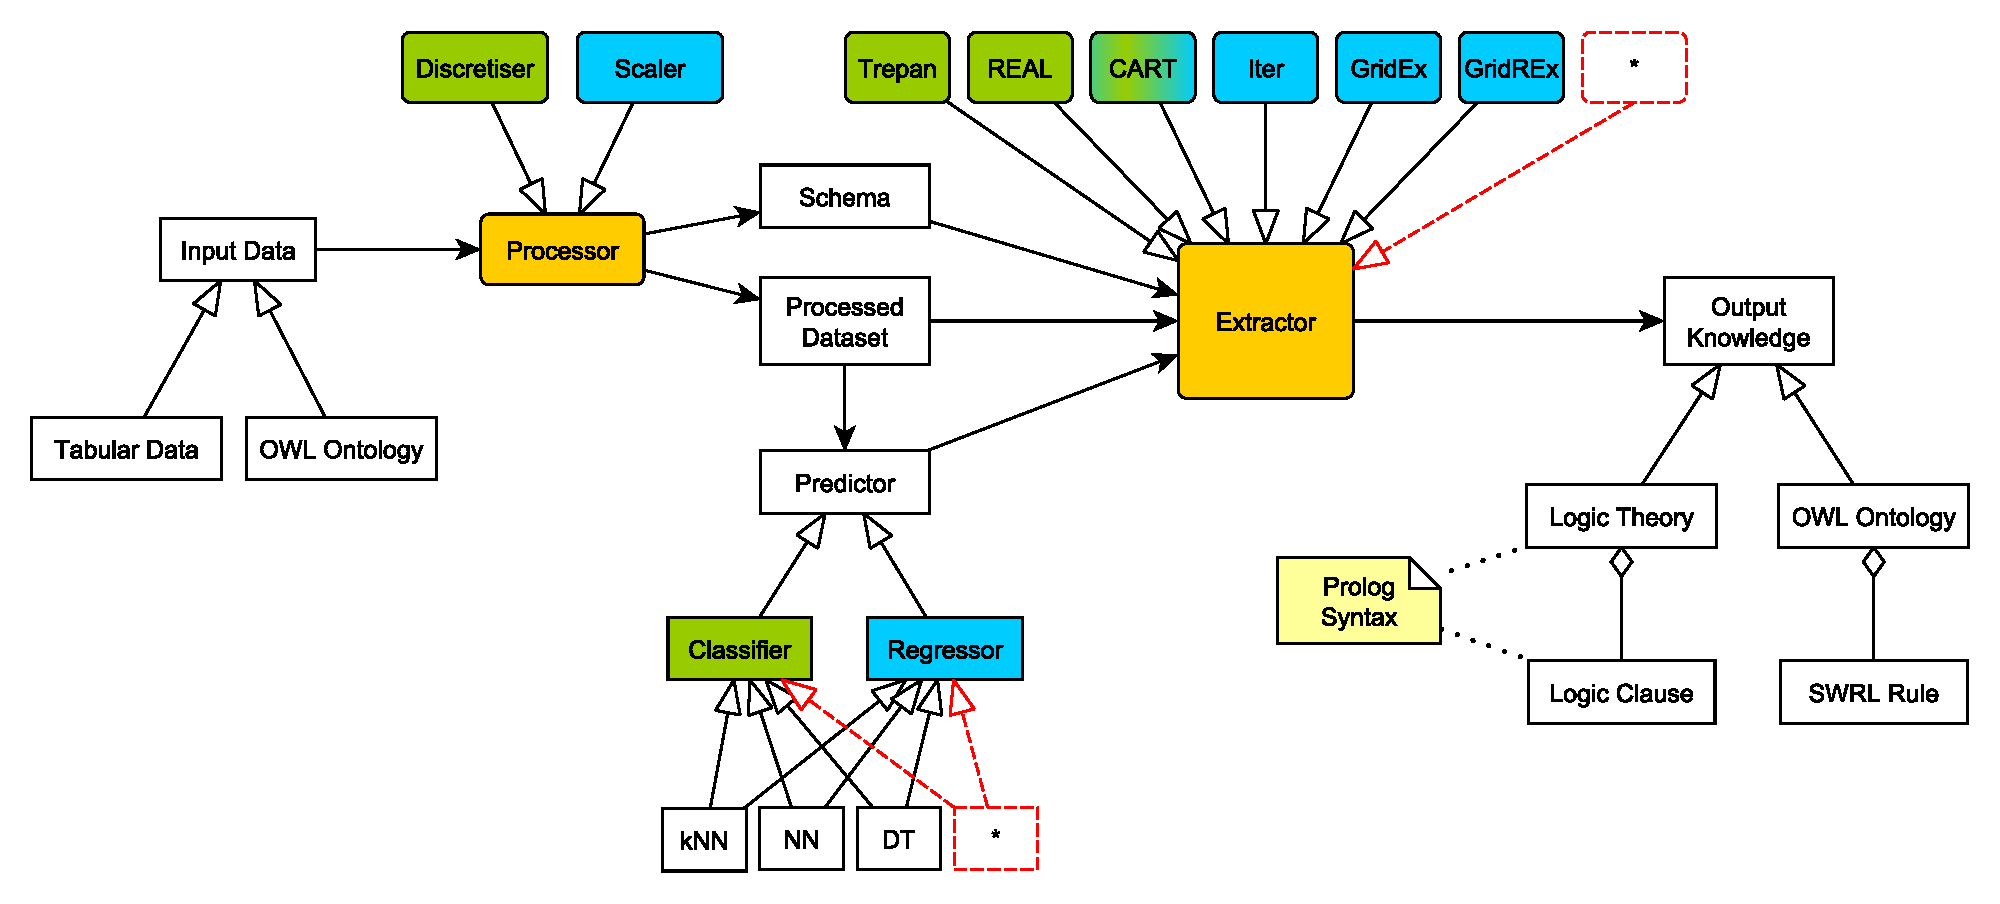
\includegraphics[width=.9\linewidth]{figures/Psyke.pdf}
	\caption{\psyke{} design.}
	\label{fig:psyke-design}
\end{figure}

% !TeX root = ia-2021-psyke.tex

\begin{table}
	\caption{Summary of the knowledge-extraction algorithms supported by \psyke{}.}
	\labeltab{psyke}
	\begin{tabular}{llllll}
		\toprule
		Extraction & Ref. & Task & Input Features & Output type & Knowledge Shape \\
		Algorithm & & & & & \\
		\midrule
		\real{} & \cite{craven1994using} & Classification & Binary & String label & Rule list \\
		\trepan{} & \cite{craven1996extracting} & Classification & Binary & String label & Decision tree \\
		\iter{} & \cite{huysmans2006iter} & Regression & Continuous & Numerical constant & Rule list \\
		\gridex{} & \cite{gridex-extraamas2021} & Regression & Continuous & Numerical constant & Rule list \\
		\gridrex{} & \cite{gridrex-kr2022} & Regression & Continuous & Regression law & Rule list \\
		\cart{} & \cite{breiman1984classification} & Classification, & Any & String label, & Decision tree \\
		& & Regression & & Numerical constant & \\
		\bottomrule
	\end{tabular}
\end{table}


The \psyke{}~\cite{psyke-woa2021,psyke-ia2022} software library is a Python framework providing general-purpose support to SKE.
%
It can be exploited to obtain logic rules from BB classifiers and regressors via several pedagogical extraction methods.
%
Its unified API allow users to select the most adequate procedure with few lines of code, also allowing fast comparison between different alternatives.
%
At the time of writing, \psyke{} supports 6 state-of-the-art SKE algorithms, reported on the top of \Cref{fig:psyke-design} (see \Cref{tab:psyke} for further details), allowing researchers and data scientists to exploit them without the need to implement and test them.

As shown in \Cref{fig:psyke-design}, the \psyke{} design is developed around the notion of \emph{extractor}, intended as any algorithm accepting as input a ML predictor (classifier or regressor) together with the data set used to train it, and providing as output a \emph{theory} of \emph{logic} rules extracted from the predictor.
%
\psyke{} extractors need additional information about the data set to give more human-interpretability to the extracted knowledge.
In particular, a schema of the data set can be given as input to formally describe input and output feature names and types.

\psyke{} also exhibits utilities to manipulate the data set and perform feature engineering, for instance procedures to discretise or scale continuous features and to one-hot encode discrete/discretised features.
%
In addition, there are automatic procedures to select the optimal parameters of the extractors, which manual tuning may be challenging for human users.

As for the knowledge provided in output by extractors, it is possible to choose between two options:
\begin{inlinelist}
	\item a Prolog theory composed of human-intelligible clauses, possibly simplified to ease readability;
	\item an OWL ontology having agent-interpretable SWRL rules, to pursue interoperability between intelligent agents~\cite{psyke-extraamas2022}.
\end{inlinelist}
%
Input data as well may follow Semantic Web encoding, so \psyke{} extractors accept tabular data or knowledge graphs stored in OWL ontologies.

\section{Hypercube-based methods}\label{sec:contribution}

In this section, we provide a general model of hypercube-based knowledge extractors.
%
We then delve into the details of different algorithms from the literature, and we discuss how they match the model.

\subsection{Unified Model}

Hypercube-base extraction methods are \emph{pedagogical} extraction procedures which can operate on trained ML predictors of any sort.
%
They consider the predictor $P$ undergoing extraction as an oracle to be queried multiple times, in order to find a partitioning $H_1 \cup \ldots \cup H_n$ of its input space $\mathcal{X}$ such that the output space $\mathcal{Y}$ can be concisely and correctly expressed for each partition.
%
Hence, they extract knowledge in the form of rule lists or trees, where each rule carries attempts to describe the outcome of $P$ in a particular hypercube $H_i \subseteq \mathcal{X}$. 
%
More formally: 
%
\[ \mathbf{x} \in H_i \rightarrow (~\mathbf{y} = f_i(\mathbf{x})~) \]  
%
to be read as ``if the input vector $\mathbf{x} \in \mathcal{X}$ is in some hypercube $H_i$, then the prediction $\mathbf{y} \in \mathcal{Y}$ is $f_i(\mathbf{x})$''.
%
Notice that each hypercube $H_i$ is a partition of the input space $\mathcal{X}$, and it comes with a function $f_i$ approximating $P$ within that hypercube.
%
More formally: $f_i(\mathbf{x}) \approx P(\mathbf{x}),~\forall \mathbf{x} \in H_i$.

Regardless of its technical details, hypercube-based extraction procedures should then attempt to select hypercubes and local approximation functions in such a way to maximise the fidelity of the overall rule set/list w.r.t. $P$.
%
To do so, they follow a quite liner workflow, may be roughly summarised in 3 steps, namely:
%
\begin{enumerate}
	\item partition the input space into disjoint hypercubes $H_1 \cup \ldots \cup H_n$, following some strategy and according to defined constraints;
	% %
	% \begin{itemize}
	% 	\item e.g. one may be willing to minimise $n$ while maximising the size of each $H_i$
	% \end{itemize}
	\item approximate the prediction of $P$ for each hypercube $H_i$, via some function $f_i$; and
	% %
	% \begin{itemize}
	% 	\item e.g. one may be willing to maximise the similarity among $P$ and $f_i$ in $H_i$
	% \end{itemize}
	\item create a rule set where each rule \emph{concisely} represents $H_i$ and $f_i$ to describe the behaviour of $P$ in $H_i$.
\end{enumerate}
%
% It is important to notice that hypercube-based extractors produce as output a predictive rule per found partition.

In the following, we delve into the details of all such phases, individually.

\subsubsection{Input space partitioning}

Input space partitioning is a recursive computation aimed at finding the optimal amount, shape and size of hypercubes w.r.t.\ some \emph{desiderata}, such as:
%
\begin{inlinelist}
	\item covering the whole input space;
	\item obtaining disjoint regions;
	\item minimising the regions' amount;
	\item maximising the similarity amongst the samples inside single regions;
	\item minimising the predictive error correlated to each partition.
\end{inlinelist}

It is not possible to satisfy all these conditions at once, especially when dealing with high-dimensional data sets.
%
For this reason, some requirements may be relaxed.
%
For instance, the input space coverage may be limited only to \emph{interesting} hypercubes, neglecting the others.
%
A hypercube is considered as `interesting' if it contains training samples, as it may have a role to play in drawing future predictions.

Alternatively, the partitioning process may terminate after a predefined number of iterations, as some existing algorithms actually do.
%
However, this may lead to the indiscriminate exclusion of some regions of the input space that, conversely, are not negligible.
%
This may result in the impossibility for the explainable model to provide predictions for a subset of input instances.

Non-contiguous hypercubes may be relaxed into hierarchical or fuzzy regions, possibly mapped into non-overlapping rules, in order to have unambiguous output predictions.

\paragraph{Similarity and fidelity}

The amount of the hypercubes an input space is partitioned into may greatly impact the interpretability of the final symbolic model.
%
In fact, hypercube-based methods will output as many rules as the hypercubes they have partitioned the input space into---and of course more (or more complex) rules implies lower readability for the human reader.

Along this line, the capability of grouping together similar samples into a single hypercube is quintessential to support the creation of few, general, and simple rules %that capture well the average behaviour of instances belonging to the same region.
which capture the behaviour of the original predictor with high fidelity.
%
This corresponds to
%
\begin{inlinelist}
	\item data points from the same hypercube drawing \emph{similar} predictions, and to
	\item those predictions having a high \emph{fidelity} (or, equivalently, low error rates) w.r.t. to the predictor undergoing extraction.
\end{inlinelist}
%
Accordingly, here we delve into the details of how 
%
\begin{inlinelist}
	\item similarity amongst data points from \emph{contiguous} hypercubes, as well as
	\item predictive errors amongst a candidate rule and the underlying predictor
\end{inlinelist}
%
can be assessed in many different scenarios.

\subparagraph{Similarity amongst instances}

Partitions of an input space may be considered similar according to the following definitions:
%
\begin{description}
	\item[input closeness] if the input variables of both subregions have values ranging in similar domains, as for the case of adjacent disjoint or overlapping regions;
	\item[output closeness] if the output associated to the instances in the 2 subregions may be defined similar.
\end{description}
%
While it is straightforward to check input closeness (e.g., through Euclidean distance), dealing output closeness requires taking into account the learning problem at hand.

As far as classification is concerned, we may consider two hyper-cubes $H_1$ and $H_2$ as \emph{output-close} w.r.t. a predictor $P$ if (and only if) the most frequent output class is the same in both hypercubes.
%
More formally:
%
\begin{equation}\label{eq:simClass}
	H_1 \stackrel{P}{\approx} H_2 \Leftrightarrow \text{mode}(P(H_1)) = \text{mode}(P(H_2))\,
\end{equation}
%
where, by $\text{mode}(\cdot)$ we denote the statistical operator returning the most frequent item over in a set, and $P(H)$ is a notational abuse for $\{ P(\textbf{x}) : \textbf{x} \in H \}$.

Conversely, in the case of regression with constant outputs, output-similarity may be expressed as a function of the absolute difference between the mean output predictions performed by the predictor $P$ on the two hypercubes $H_1$ and $H_2$:
%
\begin{equation}\label{eq:simRegK}
	H_1 \stackrel{P}{\approx} H_2 \Leftrightarrow |\text{mean}(P(H_1)) - \text{mean}(P(H_2))| < \theta\,
\end{equation}
%
where $\theta$ is a parameter defining the strictness of the similarity criterion.

Of course, this definition \ref{eq:simRegK} is not suitable to capture the similarity amongst hypercubes characterised by a high variability of $P$.
%
In this case a more complex solution is required:
%
\begin{equation}\label{eq:simRegLin}
	H_1 \stackrel{P}{\approx} H_2 \Leftrightarrow \text{mae}(f_{1,2}, H_1 \cup H_2) \leq (\text{mae}(f_1, H_1) + \text{mae}(f_2, H_2)) / 2 \,
\end{equation}
%
where $\text{mae}(f, H)$ is the mean absolute error of the linear function $f$ in approximating the input/output relationship for data instances in $H$.
%
In other words, $H_1$ and $H_2$ are output-similar if it is possible to
%
\begin{inlinelist}
	\item merge the two hyper-cubes, and to
	\item find a linear combination of the input variables representing the input/output relationship of the merged region, and
	\item the predictive performance of such linear combination is better than the average performance of the linear functions $f_1, f_2$ associated to the corresponding separated subregions.
\end{inlinelist}

\begin{figure*}[tb]\centering
	\subfloat[Classification labels.]{
		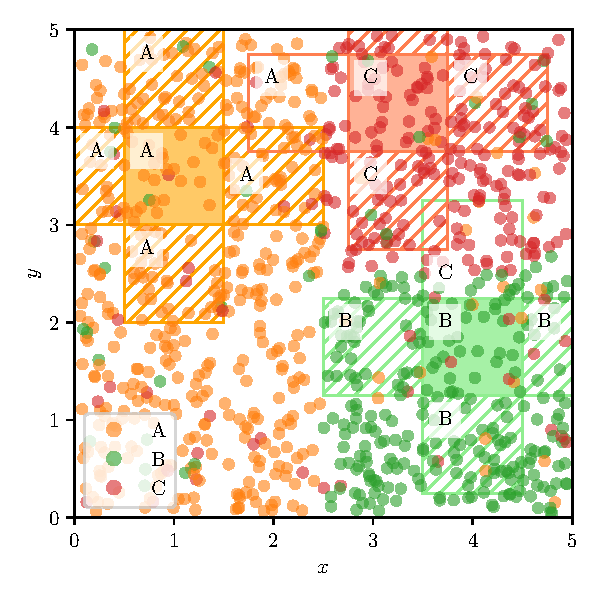
\includegraphics[width=0.295\linewidth]{figures/class-sim.pdf}\label{fig:gs1}
	}
	\subfloat[Constant outputs.]{
		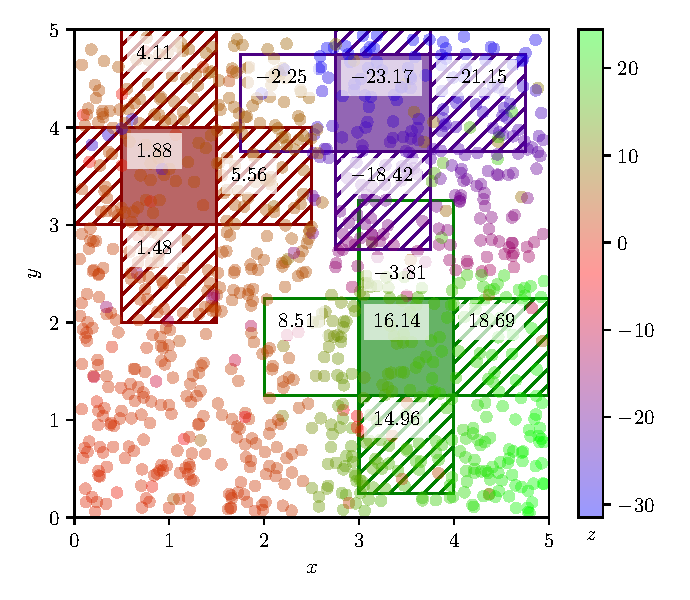
\includegraphics[width=0.34\linewidth]{figures/const-sim.pdf}\label{fig:gs2}
	}
	\subfloat[Regression laws.]{
		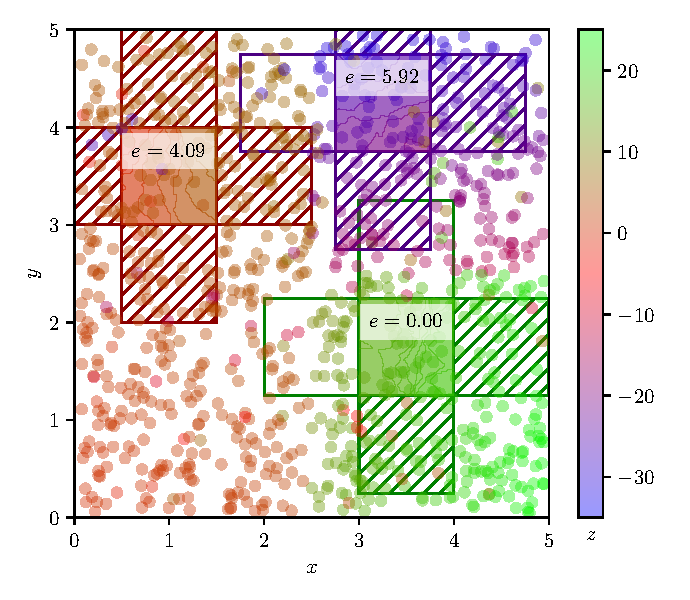
\includegraphics[width=0.34\linewidth]{figures/regr-sim.pdf}\label{fig:gs3}
	}
	\caption{Two-dimensional example of different similarities calculated for generalised extractors. Hatched regions are suitable to be merged with the adjacent one (coloured background).}\label{fig:general-sim}
\end{figure*}


For example, in \Cref{fig:general-sim} we report examples of similarity assessments calculated for a generalised extractor applied to a classification task (\Cref{fig:gs1}) and to a regression task (\Cref{fig:gs2,fig:gs3}).
%
Figures concerning the regression task represent constant and non-constant extractor outputs, respectively.
%
The example assumes a 2-dimensional data set with continuous input features both ranging in the interval [0, 5].
%
In the figures, hypercubes to be expanded/merged are those having coloured background.
%
Possible adjacent hypercubes to be joined to them are represented as hypercubes having no background.
%
Adjacent hypercubes that are similar to the hypercubes to be expanded are represented with hatched background.
%
It worths noting that for the example depicted in \Cref{fig:gs2} a similarity threshold $\theta$ equal to 5.0 has been chosen.
%
In \Cref{fig:gs3} the predictive errors corresponding to the adjacent hypercubes as well as the calculated errors of the possible merged regions are omitted to keep the image clearer.

\subparagraph{Predictive error assessment}

A generalised metrics is necessary to assess the predictive performance of a set of rules for both classifications and regressions.
%
We propose as error function for a rule set $R$ applied to a data set $D$ the following:
%
\begin{equation}\label{eq:error}
	\text{error}(R, D) = 
	\begin{cases}
		\text{mae}(R, D) & \text{(regression)}\\
		1 - \text{accuracy}(R, D) & \text{(classification)}\\
	\end{cases}\,
\end{equation}
%
where $\text{mae}(R, D)$ and $\text{accuracy}(R, D)$ are the mean absolute error and the classification accuracy score, respectively, calculated on the output predictions obtained via the rules in $R$, for the data set $D$, and w.r.t.\ the expected outputs for $D$.

\begin{figure*}[tb]\centering
	\subfloat[Classification labels.]{
		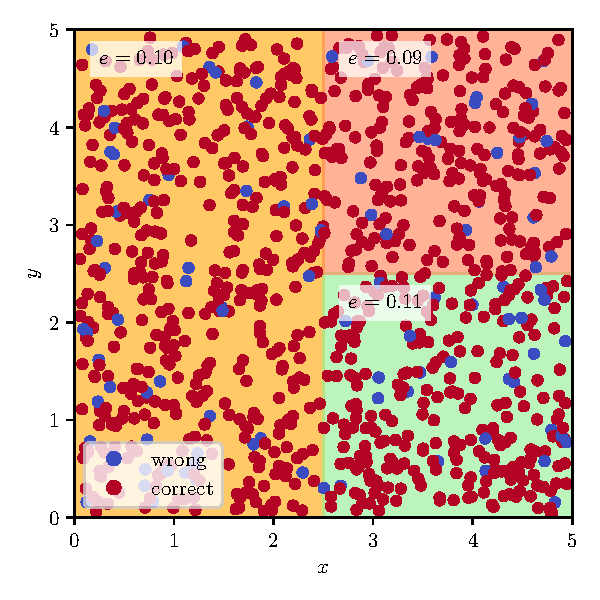
\includegraphics[width=0.295\linewidth]{figures/class-err.pdf}\label{fig:ge1}
	}
	\subfloat[Constant outputs.]{
		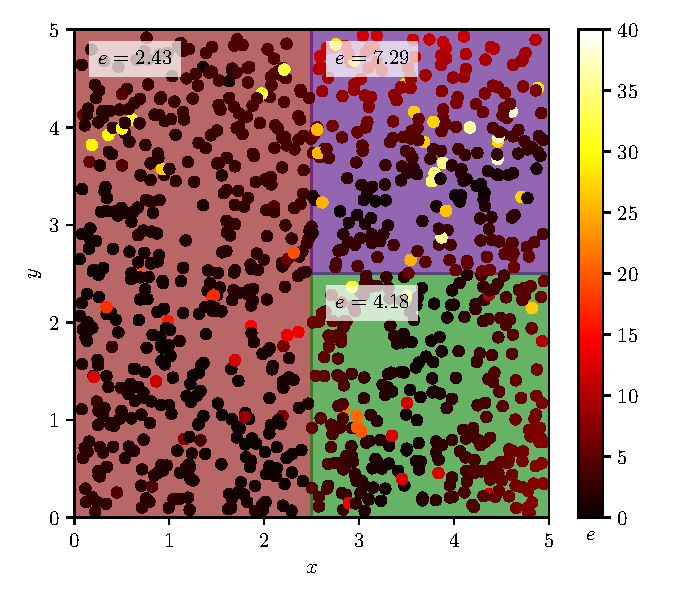
\includegraphics[width=0.34\linewidth]{figures/const-err.pdf}\label{fig:ge2}
	}
	\subfloat[Regression laws.]{
		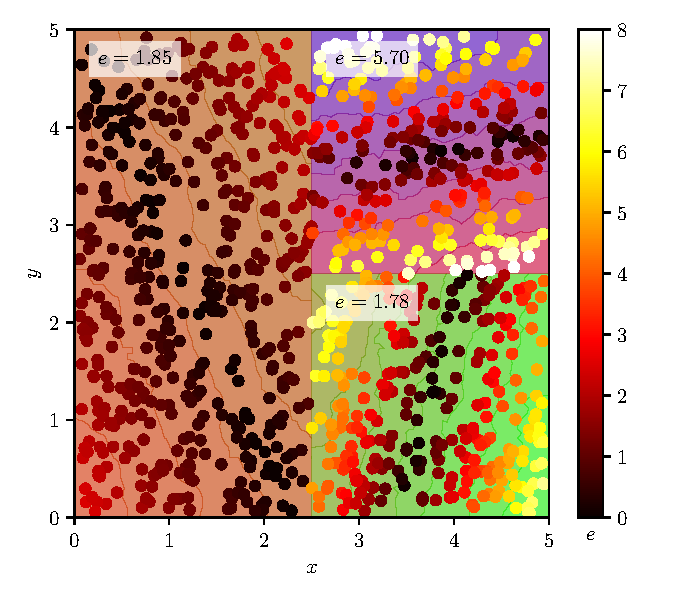
\includegraphics[width=0.34\linewidth]{figures/regr-err.pdf}\label{fig:ge3}
	}
	\caption{Two-dimensional example of different predictive errors measured for generalised extractors. Hatched regions are suitable to be merged with the adjacent one (coloured background).}\label{fig:general-error}
\end{figure*}


In \Cref{fig:general-error} we report some examples of predictive errors measured for a generalised extractor by assuming a 2-dimensional data set with continuous input features both ranging in the [0, 5] interval.
%
\Cref{fig:ge1,fig:ge2,fig:ge3} represent a classification task and two regression tasks, respectively.
%
The first regression task is approximated by the extractor with constant outputs, whereas the second is associated to non-constant outputs.
%
The predictive error is reported as misclassifications in the first case and absolute error in the others.
 
\subsubsection{Approximating predictions}

As for the approximation of output predictions associated with each hypercube, they are usually computed on the basis of the predictions provided by the underlying black box when applied to an \emph{extended} training set.
%
The extended training set may consist of the original data the predictor has been trained upon -- or a subset of it --, possibly augmented with some further data.
%
Data augmentation via random input samples is useful to attain higher predictive performance, provided that the predictor is used as an oracle to compute the corresponding expected outputs.

Provided that the input space has been adequately partitioned into several hypercubes, the prediction associated with each hypercube may consist of 
%
\begin{inlinelist}
	\item a constant numerical value (e.g., \iter{}, \gridex{}, \cart{}) or, 
	\item a linear combination of the input variables (e.g., \cart{}).
\end{inlinelist}
%
The latter option, in particular, is well-suited for regression tasks, while the former may support both classification and regression tasks.

To choose the best output value corresponding to each hypercube, one may either 
%
\begin{inlinelist}
	\item aggregate the predictions corresponding to all available points in that hypercube -- e.g. via the `mean', `mode', or `median' statistical aggregation functions --, or
	\item fit a local function \emph{locally} approximating the predictor in that hypercube.
\end{inlinelist}
%
Again, which option is better really depends on the learning task the underlying predictor has been designed for.
%
% The aggregation level of the computation depends on the hypercube associated to the rule.
% %
% Indeed, usually these computations are performed by considering only training instances \emph{inside} a cube, so the resulting rule is \emph{local}.
% %
% A factorisation of the common operations for both scenarios (constant and non-constant outputs) highlights that the creation of output values for extractors dedicated to regression tasks only differs in the raw aggregated computation described above.
% %
% As a consequence, the two possible computations may be exchanged without introducing any other alteration in a generic extractor, making it more versatile.

% It is possible to enlarge the applicability scope of these extractors to classification tasks thanks to the following consideration.
% %
% A classification rule based on a hypercube may be associated to a constant output value, that is the string label to be provided as prediction for every instance inside the cube.
% %
% The label may trivially be the most common label predicted by the underlying predictor applied to all the instances inside the cube.
% %
% This generalisation enable the adoption for classification tasks of SKE techniques explicitly designed for regression.

\begin{figure*}[tb]\centering
	\subfloat[Classification labels.]{
		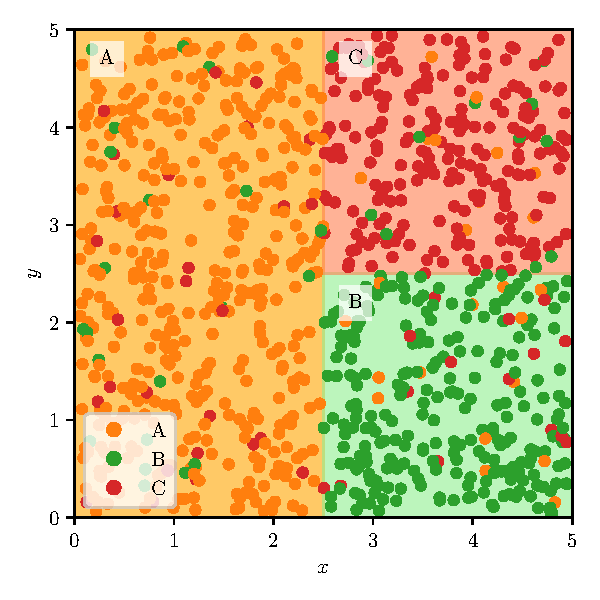
\includegraphics[width=0.295\linewidth]{figures/class.pdf}\label{fig:gp1}
	}
	\subfloat[Constant outputs.]{
		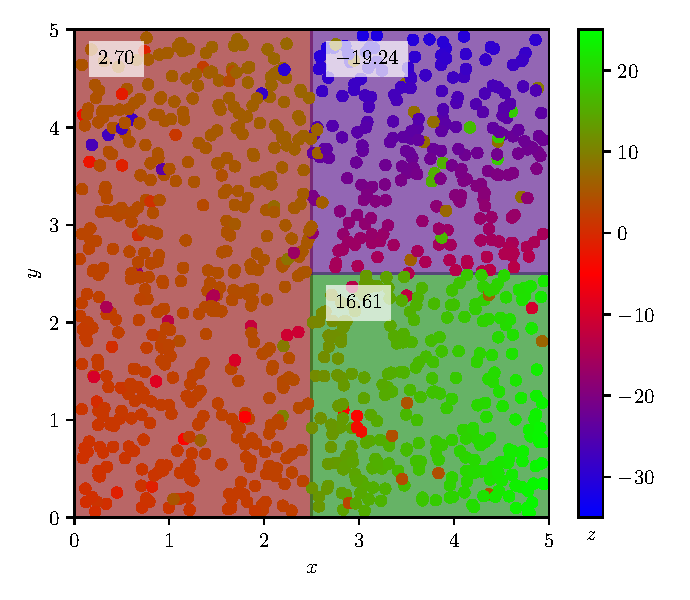
\includegraphics[width=0.34\linewidth]{figures/const.pdf}\label{fig:gp2}
	}
	\subfloat[Regression laws.]{
		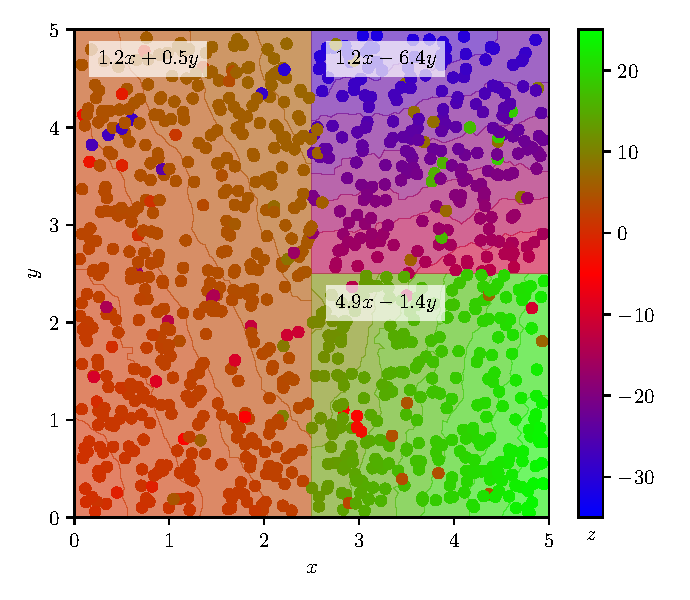
\includegraphics[width=0.34\linewidth]{figures/regr.pdf}\label{fig:gp3}
	}
	\caption{Two-dimensional example of different predictions provided by generalised extractors.}\label{fig:general-pred}
\end{figure*}


In \Cref{fig:general-pred}, we report examples of predictions provided by a generalised extractor.
%
As for the previous examples, a 2-dimensional data set with continuous input features both ranging in the [0, 5] interval is assumed.
%
\Cref{fig:gp1,fig:gp2,fig:gp3} show a classification task and two regression tasks, respectively, where the former regression task is approximated by the extractor with constant outputs.
%
The background colour represents the output provided by the extractor.

\subsubsection{Output rule creation}\label{ssec:rule}

After selecting a set of input space regions and one output decision for each of them, hypercube-based extractors build a set of rules where each one is composed of a precondition and a postcondition.
%
The precondition is a formal description of a single input region in terms of individual features, for instance by means of value inclusion inside an interval.
%
Hypercubic $n$-dimensional regions may be described through the conjunction of (at most) $n$ interval inclusion conditions.
%
On the other hand, the postcondition is simply the decision calculated for the region on the basis of the task at hand, as previously described.
%
Thus, extracted human-readable logic rules generally have the following format:
%
\begin{equation*}
	\text{Output is ~} C \text{~ if ~} X_1 \in [l_1, u_1], X_2 \in [l_2, u_2], ..., X_n \in [l_n, u_n],
\end{equation*}
%
where $O$ is the output decision and $X_1, X_2, ..., X_n$ are input variables assuming values included in the intervals described by corresponding lower-bounds $l_i$ and upper-bounds $u_i$.

\subsection{Comparison of Existing Methods}

In the following a comparison between the hypercube-based SKE algorithms cited in \Cref{sec:experiments} -- namely \iter{} and \gridex{} -- is provided to give a practical demonstration of our methodology.
%
Differences in the input space partitioning and in the decision approximation are highlighted in particular.
%
Output rules are lists of logic rules in both cases, following the convention described in \Cref{ssec:rule}.
%
It worths noting that both algorithms assume input features to be continuous and may be applied to any kind of BB predictor, being pedagogical SKE methods.

\paragraph{\iter}

The \iter{} algorithm~\cite{huysmans2006iter} is based on the iterative creation and expansion of hypercubes inside the input feature space, until a maximum number of iterations is reached or, otherwise, the whole input space is covered.
%
The expansion may terminate also if it is not possible to further expand the hypercubes.
%
In those cases additional cubes may be created to cover the remaining space.

\iter{} has been designed limitedly to regression tasks and it performs averaging operations to associate output values to hypercubes.
%
Indeed, for each cube, \iter{} selects all the training samples inside it and calculates the mean prediction by using the underlying BB as an oracle.
%
If the training samples are not enough to satisfy the minimum amount specified by the user, extra random samples are generated and predicted together with the others.

\iter{} also takes advantage of a similarity criterion to expand the hypercubes.
%
In particular, at every iteration all the possible expansions around each cube are considered, but only one is performed, i.e., the one capable of expanding a cube towards the most similar input space region.
%
Similarity is calculated via mean absolute difference between the output values of the cubes to be expanded and the eligible cubes around them.

\paragraph{\gridex{}}

The \gridex algorithm~\cite{gridex-extraamas2021} may be considered as an extension of \iter{} aimed at overcoming its major drawback, i.e., the non-exhaustivity of its output rules.
%
\gridex{} achieves this goal because it is exhaustive by design.
%
Differently from \iter{}, \gridex{} adopts a top-down approach to split the input feature space into hypercubes.
%
It iteratively partitions the \emph{whole} space according to some defined strategy, marking at each iteration if the created partitions are \emph{negligible} (i.e., they contain no training samples, so they are discarded since it is not relevant to have rules associated to them), \emph{eligible} for further partitioning (if they contain samples that are not enough \emph{similar}), or \emph{permanent} (otherwise, if they contain similar training instances and, thus, these cubes should have a good predictive performance).
%
Strategies to split the input space are \emph{fixed}, if the user specifies for each iterations how many partitions have to be performed along all the input dimensions, or \emph{adaptive}, if the number of splits is determined through the relevance of each input feature w.r.t.\ the output variable.
%
Since \gridex{} has been designed exclusively for regression tasks, as \iter{}, also in this case output decisions are calculated via local averaging calculations and actual regression rules are not supported.

Similarity between samples is assessed through the output value standard deviation of all the instances included inside a hypercube.
%
If the standard deviation is below a user-defined threshold, then the cube only contains similar samples and it is no further partitioned.
%
Otherwise, \gridex{} attempts to split the cube in smaller regions, possibly enclosing more similar samples.
%
Since the readability of the output model depends on the number of extracted rules, it is of paramount importance to keep it as low as possible.
%
For this reason a merging phase is performed after every splitting iteration as an optimisation to reduce the number of rules.
%
Indeed, adjacent cubes are pairwise merged according to a similarity criterion on the contained samples.
%
The merging phase is iterative: at each step are merged only the two adjacent cubes resulting in the merged hypercube having the lowest standard deviation, and it terminates when it is not possible to further merge cubes without exceeding the standard deviation user-defined threshold.

A first attempt to apply the generalisation proposed in this work to \gridex{}, in order to support regression rules as output decisions, can be found in the \gridrex{}~\cite{gridrex-kr2022} algorithm.
%
Indeed, it is able to extract fully regressive rules, having as postconditions a linear combination of the input variables.
%
All the other details are identical to those described for \gridex{}, but it is able to achieve better predictive performance, fidelity and readability than \gridex{}

\section{Case Study: \psyke}\label{sec:experiments}

Here, we exemplify the effectiveness of hypercube-based methods, as implemented by the \iter{} and \gridex{} extraction algorithms.
%
Both such methods are designed for regression and here applied to classification tasks.
%
\cart{} is used as benchmark to assess the predictive performance of the modified extractors, since it is a state-of-the-art procedure directly applicable to data sets described by continuous features, without prior discretisation.
%
All the adopted implementations are included in the \psyke{} framework\footnotemark.

\footnotetext{Code of experiments is available at \url{https://github.com/psykei/psyke-python}}

Experiments are executed on the well-known Iris data set\footnotemark.
%
\footnotetext{\vurl{https://archive.ics.uci.edu/ml/datasets/iris}}
%
The data set is composed of 150 instances corresponding to Iris flower individuals.
%
Each instance is described by 4 continuous input features (i.e., petal and sepal width and length of the Iris exemplary) and a categorical class label (i.e., the species of the exemplary).
%
Three different species are present in the Iris data set (namely, Setosa, Virginica, and Versicolor) and they are equally balanced (50 individuals per species).

The experiments are carried out as follows:
%
\begin{inlinelist}
	\item the data set is randomly split into training and test sets, of equal size;
	\item a $k$-nearest neighbour classifier is trained on the training set;
	\item three different extractors are used to extract symbolic rules out of that classifier;
	\item the predictive performance of both the classifier and the extracted rules are graphically compared -- in terms of decision boundaries --, and numerically assessed---in terms of accuracy and F1 scores. In the case of the extracted rules, fidelity and readability measurements are performed as well.
\end{inlinelist}
%
It worths noticing that the training set is used only to train the models.
%
Conversely, the test set is used only to assess the predictive performance of predictor and extractors.
%
Both sets are constant for each experiment, to better compare the performance under the same conditions.
%
The fidelity of the extracted rules (w.r.t.\ the predictor they have been extracted from) is assessed as well, via the same metrics adopted for the predictive performance.
%
Finally, the output knowledge readability is expressed as number of extracted rules.

\subsection{Predictor training}

% !TeX root = woa-2021-psyke.tex

\begin{table}
	\caption{Comparison between accuracy and F$_1$ scores for several $k$-NN predictors having different values for $k$.}
	\label{tab:predictor}
	\begin{tabular}{c|c|ccc}
		\toprule
		& Accuracy & \multicolumn{3}{c}{F$_1$ score}\\
 		$k$ & score & Setosa & Virginica & Versicolor \\
		\midrule
		3 & 0.93 & 1.00 & 0.89 & 0.92 \\
		5 & 0.96 & 1.00 & 0.94 & 0.95 \\
		7 & 0.96 & 1.00 & 0.94 & 0.95 \\
		\textbf{9} & \textbf{0.97} & \textbf{1.00} & \textbf{0.96} & \textbf{0.97} \\
		11 & 0.95 & 1.00 & 0.91 & 0.94 \\
		13 & 0.93 & 1.00 & 0.89 & 0.92 \\
		15 & 0.93 & 1.00 & 0.89 & 0.92 \\
		17 & 0.96 & 1.00 & 0.94 & 0.95 \\
		\bottomrule
	\end{tabular}
\end{table}

Extraction techniques require an underlying BB to be used as an oracle.
%
For this reason we trained and compared several $k$-NN classifiers, with different values for the $k$ hyper-parameter.
%
Details about the accuracy and F1 scores measured for each model are reported in \Cref{tab:predictor}.
%
The best predictive performance is achieved by the 9-NN.
%
Consequently, in the following all the discussed extractors are applied to it.
%
The decision boundaries of the selected 9-NN are reported in \Cref{fig:knn}.

\subsection{\cart{}}

% !TeX root = woa-2021-psyke.tex

\begin{table}
	\caption{Accuracy and F1 scores observed for \cart{} applied to the 9-NN classifier. Fidelity measurements are reported inside the parentheses.}
	\label{tab:cart}
	\begin{tabular}{c|c|ccc}
		\toprule
		& Accuracy & \multicolumn{3}{c}{F1-score}\\
 		\# of rules & score & Setosa & Virginica & Versicolor \\
		\midrule
		3 & 0.95 (0.95) & 1.00 (1.00) & 0.91 (0.91) & 0.94 (0.94) \\
		\bottomrule
	\end{tabular}
\end{table}


The \cart{} extractor is applied to the 9-NN classifier to extract human-intelligible knowledge in Prolog syntax, without discretising the input data set.
%
Differently from \iter{} and \gridex{}, \cart{} is able to work upon discretised data sets too.
%
Training the model with a maximum leaf amount of 3 gives the following theory, composed of 3 rules---namely, one per each possible class of the Iris data set.

\prologimport{listings/iris-rules-cart.pl}

The theory is always exhaustive, since it is always possible to find a leaf classifying an instance.
%
Numerical assessments about the predictive performance and fidelity of the theory extracted with \cart{} are reported in \Cref{tab:cart}.
%
The input space partitioning induced by the theory is reported in \Cref{fig:cart}.
%
In this example, only petal width and length are considered to assign class labels to input instances.

\subsection{\iter{}}

% !TeX root = woa-2021-psyke.tex

\begin{table}
	\caption{Comparison between accuracy and F1 scores for several instances of \iter{} having different hyper-parameters. Fidelity measurements are reported inside the parentheses.}
	\label{tab:iter}
	\begin{tabular}{c|c|c|c|c|ccc}
		\toprule
		Update & Starting & Min. & \# of & Accuracy & \multicolumn{3}{c}{F1-score}\\
 		size & points & examples & rules & score & Setosa & Virginica & Versicolor \\
		\midrule
		0.10 & 1 & 75 & 4 & 0.84 (0.87) & 1.00 (1.00) & 0.81 (0.84) & 0.78 (0.82) \\
		0.10 & 1 & 150 & 4 & 0.84 (0.87) & 1.00 (1.00) & 0.81 (0.84) & 0.78 (0.82) \\
		0.10 & 3 & 75 & 3 & 0.84 (0.87) & 1.00 (1.00) & 0.81 (0.84) & 0.78 (0.82) \\
		0.10 & 3 & 150 & 4 & 0.84 (0.87) & 1.00 (1.00) & 0.81 (0.84) & 0.78 (0.82) \\
		\textbf{0.07} & \textbf{1} & \textbf{75} & \textbf{3} & \textbf{0.94 (0.97)} & \textbf{1.00 (1.00)} & \textbf{0.92 (0.96)} & \textbf{0.93 (0.97)} \\
		\textbf{0.07} & \textbf{1} & \textbf{150} & \textbf{3} & \textbf{0.94 (0.97)} & \textbf{1.00 (1.00)} & \textbf{0.92 (0.96)} & \textbf{0.93 (0.97)} \\
		0.07 & 3 & 75 & 4 & 0.94 (0.97) & 1.00 (1.00) & 0.92 (0.96) & 0.93 (0.97) \\
		0.07 & 3 & 150 & 6 & 0.94 (0.97) & 1.00 (1.00) & 0.92 (0.96) & 0.93 (0.97) \\
		\bottomrule
	\end{tabular}
\end{table}


The \iter{} algorithm explain applied as well to explain the 9-NN classifier.
%
We test several hyper-parameter values in order to attain the rule list having the highest possible predictive performance and fidelity.
%
\iter{} is based on the following hyper-parameters:
%
\begin{inlinelist}
	\item the size for updating cubes, expressed as fraction of input dimension (i.e., 0.1 means a tenth of the interval between minimum and maximum values of each dimension);
	\item the number of starting points, representing the initial hypercubes;
	\item the minimum number of examples to consider in each cube;
	\item the similarity threshold between adjacent cubes, that is not relevant for classification;
	\item the maximum number of iterations, fixed to 600.
\end{inlinelist}

The results of our experiments for \iter{} are reported in \Cref{tab:iter}.
%
The best predictive performance, achieved with the parameters highlighted in bold font in the Table, correspond to the following rules.
%
\prologimport{listings/iris-rules-iter.pl}
%
The input space partitioning induced by the extracted rules is shown in \Cref{fig:iter}.

\subsection{\gridex{}}

% !TeX root = woa-2021-psyke.tex

\begin{table}
	\caption{Comparison between accuracy and F$_1$ scores for several instances of \gridex{} having different hyper-parameters. Fidelity measurements are reported inside the parentheses.}
	\labeltab{gridex}
	\begin{tabular}{c|c|c|c|ccc}
		\toprule
		& Adaptive & & Accuracy & \multicolumn{3}{c}{F$_1$ score}\\
 		Depth & strategy & \# of rules & score & Setosa & Virginica & Versicolor \\
		\midrule
		1 & (0.85, 5) & 3 & 0.87 (0.90) & 1.00 (1.00) & 0.84 (0.87) & 0.82 (0.86) \\
		\textbf{1} & \textbf{(0.85, 8)} & \textbf{3} & \textbf{0.94 (0.97)} & \textbf{1.00 (1.00)} & \textbf{0.92 (0.96)} & \textbf{0.93 (0.96)} \\
		1 & (0.85, 10) & 3 & 0.87 (0.90) & 1.00 (1.00) & 0.84 (0.87) & 0.82 (0.86) \\
		2 & (0.85, 5) & 6 & 0.89 (0.91) & 1.00 (1.00) & 0.86 (0.88) & 0.83 (0.88) \\
		2 & (0.85, 8) & 6 & 0.94 (0.97) & 1.00 (1.00) & 0.92 (0.96) & 0.93 (0.96) \\
		2 & (0.85, 10) & 6 & 0.89 (0.91) & 1.00 (1.00) & 0.86 (0.88) & 0.83 (0.88) \\
		2 & (0.75, 5) & 8 & 0.93 (0.94) & 1.00 (1.00) & 0.89 (0.91) & 0.91 (0.93) \\
		2 & (0.75, 2) & 11 & 0.69 (0.69) & 0.87 (0.87) & 0.74 (0.74) & 0.39 (0.39) \\
		\bottomrule
	\end{tabular}
\end{table}


Finally, as last step of our experiments, the \gridex{} extractor is applied to the 9-NN classifier
%
In this case as well different values for the hyper-parameters are been explored.
%
We recall that fundamental hyper-parameters for \gridex{} are
%
\begin{inlinelist}
	\item the depth of the recursive partitioning (i.e., how many iterations);
	\item the number of slices to perform at every iteration;
	\item the error threshold used to decide if further divide a hypercube, fixed to 0.1 for all experiments;
	\item the minimum number of examples to consider in each cube, here fixed to 1.
\end{inlinelist}
%
As for the number of slices to be performed, adaptive strategies are preferred to fixed strategies.
%
Experiment results concerning \gridex{} are reported in \Cref{tab:gridex}.
%
The best hyper-parameter values are highlighted in bold font.
%
The semantics of adaptive splitting strategies described by the couple $(a, b)$ is the following: all input dimensions having relevance greater than $a$ are split into $b$ subregions at each iteration.
%
All the other dimensions are not split.
%
Input feature relevance is always scaled in the [0, 1] interval.
%
Corresponding output Prolog theory and input space partitioning are reported in the following and in \Cref{fig:gridex}, respectively.

\prologimport{listings/iris-rules-gridex.pl}

Also in this case only one input feature is considered to draw predictions.
%
The partitioning is exhaustive w.r.t.\ the data set, however a small input space region is neglected since the algorithm observed no instances included in it.
%
Differently from \iter{}, \gridex{} is able to detect input dimensions that do not affect the classification.
%
In this manner all the non-relevant antecedents are dropped from the output theory, resulting in a higher human-readability.

\subsection{Discussion}

\begin{figure*}[tb]\centering
	\subfloat[9-NN{}.]{
		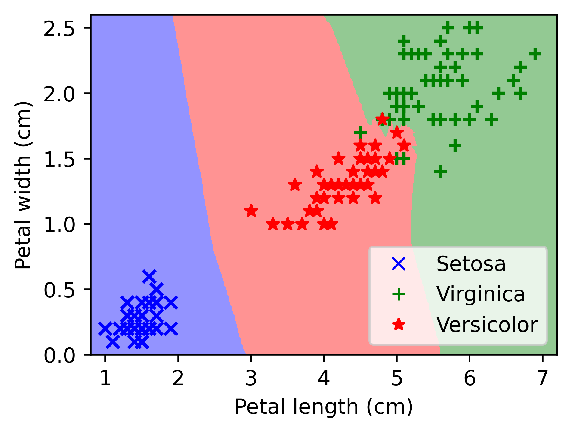
\includegraphics[width=0.45\linewidth]{figures/knn.pdf}\label{fig:knn}
	}
	\hfill
	\subfloat[\cart{}.]{
		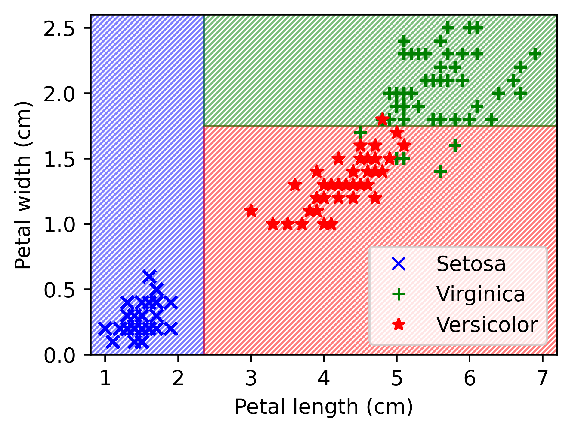
\includegraphics[width=0.45\linewidth]{figures/cart.pdf}\label{fig:cart}
	}
	\\
	\subfloat[\iter{}.]{
		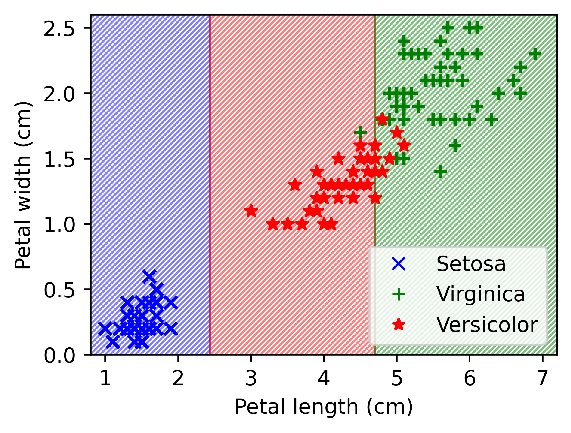
\includegraphics[width=0.45\linewidth]{figures/iter.pdf}\label{fig:iter}
	}
	\hfill
	\subfloat[\gridex{}.]{
		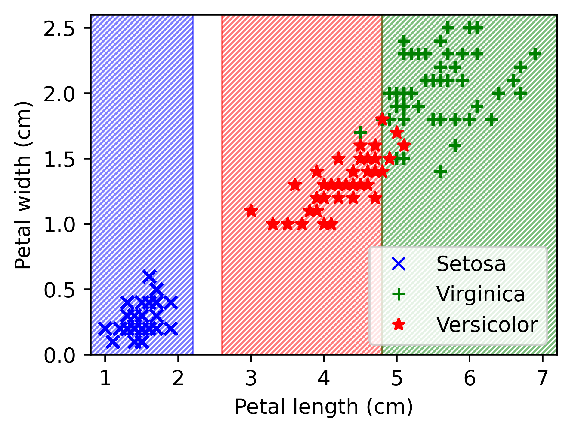
\includegraphics[width=0.45\linewidth]{figures/gridex.pdf}\label{fig:gridex}
	}
	\caption{Decision boundaries corresponding to the 4-NN predictions and to the rules extracted with 3 different extractors for the Iris data set. Only the two most relevant features are reported.}\label{fig:extractors}
\end{figure*}


In this Subsection we compare the results of \cart{}, \iter{} and \gridex{} applied to the Iris data set, all summarised in \Cref{fig:extractors}.
%
Results are compared on the basis of readability, fidelity and predictive performance, other than the decision boundaries induced by the extracted rules.
%
As for readability, all the extractors are equivalent w.r.t.\ the amount of rules, since they are able to extract one predictive rule per output class.
%
Conversely, the readability of \iter{} is hindered by the number of antecedents per rule, since it produces a constraint for each input dimension.
%
Under this perspective, \cart{} and \gridex{} are able to keep amongst the rules' conditions only those involving relevant features to perform the classification, resulting in a fourth of the total amount of antecedents w.r.t.\ \iter{}.

The decision boundaries provided by \gridex{} and \iter{} are more similar to those produced by the underlying $k$-NN, but no sensible difference in the classification accuracy are noticeable, since all extractors present a score between 0.94 and 0.95 (we recall that the 9-NN has an accuracy score equal to 0.97).
%
A similar reasoning may be performed about the extractors' fidelity, equal to 0.95 for \cart{} and to 0.97 for \iter{} and \gridex{}.

It worths noting that \gridex{} do not provide a classification rule for a small input space region, since it finds that region as negligible (because there are not data set instances belonging to it).

\section{Conclusions}\label{sec:conclusions}

In this paper we generalise a class of SKE techniques, namely hypercube-based methods, to make them suitable for classification tasks as well as regression tasks.
%
We do so by proposing a common metamodel for these methods and by concretely implementing our generalisation in the \psyke{} framework.
%
The proposed metamodel considers in which ways it is possible to relax algorithmic patterns currently adopted by hypercube-based SKE extractors in order to widen their applicability scopes.
%
Our future works will be focused on extending the proposed generalisation to a wider class of SKE techniques, to enable a higher degree of usability for SKE techniques existing in the literature.

\begin{acknowledgments}
	This paper has been partially supported by
	%
	\begin{inlinelist}
		\item the European Union's Horizon 2020 research and innovation programme under G.A.\ no.\ 101017142 (StairwAI project), and by
		\item the CHIST-ERA IV project CHIST-ERA-19-XAI-005, co-funded by the EU and the Italian MUR (Ministry for University and Research).
	\end{inlinelist}
\end{acknowledgments}

\bibliography{woa-2022-psyke}

\end{document}

%%
%% End of file
